% THIS DOCUMENT IS FOLLOWS THE VOLERE TEMPLATE BY Suzanne Robertson and James Robertson
% ONLY THE SECTION HEADINGS ARE PROVIDED
%
% Initial draft from https://github.com/Dieblich/volere
%
% Risks are removed because they are covered by the Hazard Analysis
\documentclass[12pt]{article}
\usepackage{afterpage}
\usepackage{float}
\usepackage{longtable}
\usepackage{booktabs}
\usepackage{tabularx}
\usepackage{graphicx}
\usepackage{hyperref}
\usepackage{graphicx}
\hypersetup{
    bookmarks=true,         % show bookmarks bar?
      colorlinks=true,      % false: boxed links; true: colored links
    linkcolor=red,          % color of internal links (change box color with linkbordercolor)
    citecolor=green,        % color of links to bibliography
    filecolor=magenta,      % color of file links
    urlcolor=cyan           % color of external links
}

\newcommand{\lips}{\textit{Insert your content here.}}

%% Comments

\usepackage{color}

\newif\ifcomments\commentstrue %displays comments
%\newif\ifcomments\commentsfalse %so that comments do not display

\ifcomments
\newcommand{\authornote}[3]{\textcolor{#1}{[#3 ---#2]}}
\newcommand{\todo}[1]{\textcolor{red}{[TODO: #1]}}
\else
\newcommand{\authornote}[3]{}
\newcommand{\todo}[1]{}
\fi

\newcommand{\wss}[1]{\authornote{blue}{SS}{#1}} 
\newcommand{\plt}[1]{\authornote{magenta}{TPLT}{#1}} %For explanation of the template
\newcommand{\an}[1]{\authornote{cyan}{Author}{#1}}

%% Common Parts

\newcommand{\progname}{Course Buddy} % PUT YOUR PROGRAM NAME HERE
\newcommand{\authname}{Team \#5, Overwatch League
\\ Jingyao, Qin
\\ Qianni, Wang
\\ Qiang, Gao
\\ Chenwei, Song
\\ Shuting, Shi
\\ } % AUTHOR NAMES                  

\usepackage{hyperref}
    \hypersetup{colorlinks=true, linkcolor=blue, citecolor=blue, filecolor=blue,
                urlcolor=blue, unicode=false}
    \urlstyle{same}
                                

\begin{document}

\title{Software Requirements Specification for \progname: subtitle describing software} 
\author{\authname}
\date{\today}
	
\maketitle
~\newpage

\pagenumbering{roman}

\tableofcontents

~\newpage

\section*{Revision History}

\begin{tabularx}{\textwidth}{p{3cm}p{2cm}X}
\toprule {\textbf{Date}} & {\textbf{Version}} & {\textbf{Notes}}\\
\midrule
Date 1 & 1.0 & Notes\\
Date 2 & 1.1 & Notes\\
\bottomrule
\end{tabularx}

~\\

~\newpage
\section{Purpose of the Project}
\subsection{User Business}
\lips
\subsection{Goals of the Project}
\lips
\section{Stakeholders}
\subsection{Client}
N/A
\subsection{Customer}
The primary customers are students across various levels of education, from high school to college institutions. These students are in need of a comprehensive solution to manage their overwhelming schoolwork, deadlines, and tests.
\subsection{Other Stakeholders}
\begin{itemize}
  \item \textbf{Educational Institutions}: Schools, colleges, and universities that may use this app as part of their academic toolkit.
  \item \textbf{Parents}: Concerned about their child's academic performance and well-being.
  \item \textbf{Educational Researchers}: Those interested in studying the effects of task management and its correlation with academic success.
\end{itemize}

\subsection{Hands-On Users of the Project}
\textbf{Students}: Using the application to manage their studies and academic tasks, connecting through the app's social network component for collaborative study sessions.
\subsection{User Participation}
\begin{itemize}
  \item \textbf{Initial User Involvement}
  Users will be initially involved in providing insights regarding their needs and preferences through surveys and interviews. 
  \item \textbf{User Acceptance Testing}
  Selected users will be involved in the beta testing phase to gather feedback and identify any issues or areas of improvement before the final release.
  \item \textbf{Continuous Feedback}
  Once the app is launched, user participation will continue through feedback mechanisms built into the app, allowing continuous improvement of features and user experience.
  \item \textbf{Community Engagement}
  Users can participate in community forums to discuss features, share tips, and support each other in using the app effectively
\end{itemize}

\subsection{Maintenance Users and Service Technicians}
\begin{itemize}
    \item Maintenance users and service technicians are responsible for the maintenance and optimization of the application, ensuring all features and components function as intended.
    \item They will monitor application performance, resolve any arising issues or bugs, and implement necessary updates and enhancements.
    \item Service technicians will manage the training pipeline for machine learning algorithms, ensuring the models are accurate, reliable, and up-to-date.
    \item Regular maintenance are scheduled to ensure the application's consistent performance. Critical issues are addressed immediately to minimize any disruption to users.
\end{itemize}

\section{Mandated Constraints}
\subsection{Solution Constraints}
\lips
\subsection{Implementation Environment of the Current System}
\lips
\subsection{Partner or Collaborative Applications}
\lips
\subsection{Off-the-Shelf Software}
\lips
\subsection{Anticipated Workplace Environment}
\lips
\subsection{Schedule Constraints}
\lips
\subsection{Budget Constraints}
\lips
\subsection{Enterprise Constraints}
\lips

\section{Naming Conventions and Terminology}
\subsection{Glossary of All Terms, Including Acronyms, Used by Stakeholders involved in the Project}
\begin{itemize}
    \item \textbf{UI:} User Interface - the space where interactions between humans and machines occur.
    \item \textbf{ML:} Machine Learning - a field of artificial intelligence that uses statistical techniques to give computer systems the ability to "learn" from data.
    \item \textbf{Pipeline (in ML):} A series of automated processes that allow for the streamlining of data from ingestion to processing, transformation, training, and evaluation in machine learning models.
    \item \textbf{API:} Application Programming Interface - a set of tools and definitions used to implement software applications.
    \item \textbf{HTTP:} Hypertext Transfer Protocol - an application protocol used for transferring hypermedia documents, such as HTML. It is the foundation of any data exchange on the Web.
    \item \textbf{Database:} Centralized collection of data, which can be stored, accessed, and managed easily.
    \item \textbf{Pomodoro Timer:} A time management method that uses a timer to break down work into intervals, traditionally 25 minutes in length, separated by short breaks.
\end{itemize}


\section{Relevant Facts And Assumptions}
\subsection{Relevant Facts}
\lips
\subsection{Business Rules}
\lips
\subsection{Assumptions}
\lips

\section{The Scope of the Work}

\subsection{The Current Situation}
Currently, students across various educational levels face significant challenges in managing their academic tasks and schedules effectively due to the overwhelming schoolwork. Teachers and educational institutions also seek innovative solutions to foster management skills among students and enhance their learning experiences. The existing solutions are often not comprehensive, lacking intelligent task prioritization, progress visualization, and effective time management tools.

\subsection{The Context of the Work}
The Smart Study Helper App is designed to bridge this gap by providing a user-friendly platform that combines automated task generation, intelligent task prioritization, progress visualization, and various other features. The development of this application intends to improve students' academic performance and mental well-being by reducing stress and enhancing learning experiences.
\begin{figure}[htbp]
    \centering
    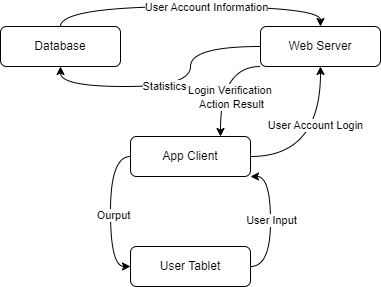
\includegraphics[width=0.7\linewidth]{Context Diagram.drawio.png} 
    \caption{Context Diagram}
    \label{fig:samplelabel}
\end{figure}

\subsection{Specifying a Business Use Case (BUC)}
\begin{itemize}
    \item \textbf{BUC Name:} Integrated Study Management
    \item \textbf{Goal:} To provide a comprehensive solution that allows students to manage their academic tasks, schedules, and study sessions effectively.
    \item \textbf{Actors:} Students, Educational Institutions, Teachers.
    \item \textbf{Preconditions:} User registration and course information uploaded or inputted.
    \item \textbf{Postconditions:} Enhanced student learning experiences, improved academic performance, reduced stress levels.
    \item \textbf{Main Success Scenario:} Students effectively use the app to manage their study tasks, leading to improved academic outcomes and reduced stress. Educational institutions and teachers observe enhanced student management skills and learning experiences.
    \item \textbf{Extensions:} Development of additional features based on user's feedback, improvement of machine learning model, larger user base.
\end{itemize}

\section{Business Data Model and Data Dictionary}
\subsection{Business Data Model}
\begin{figure}[htbp]
  \centering
  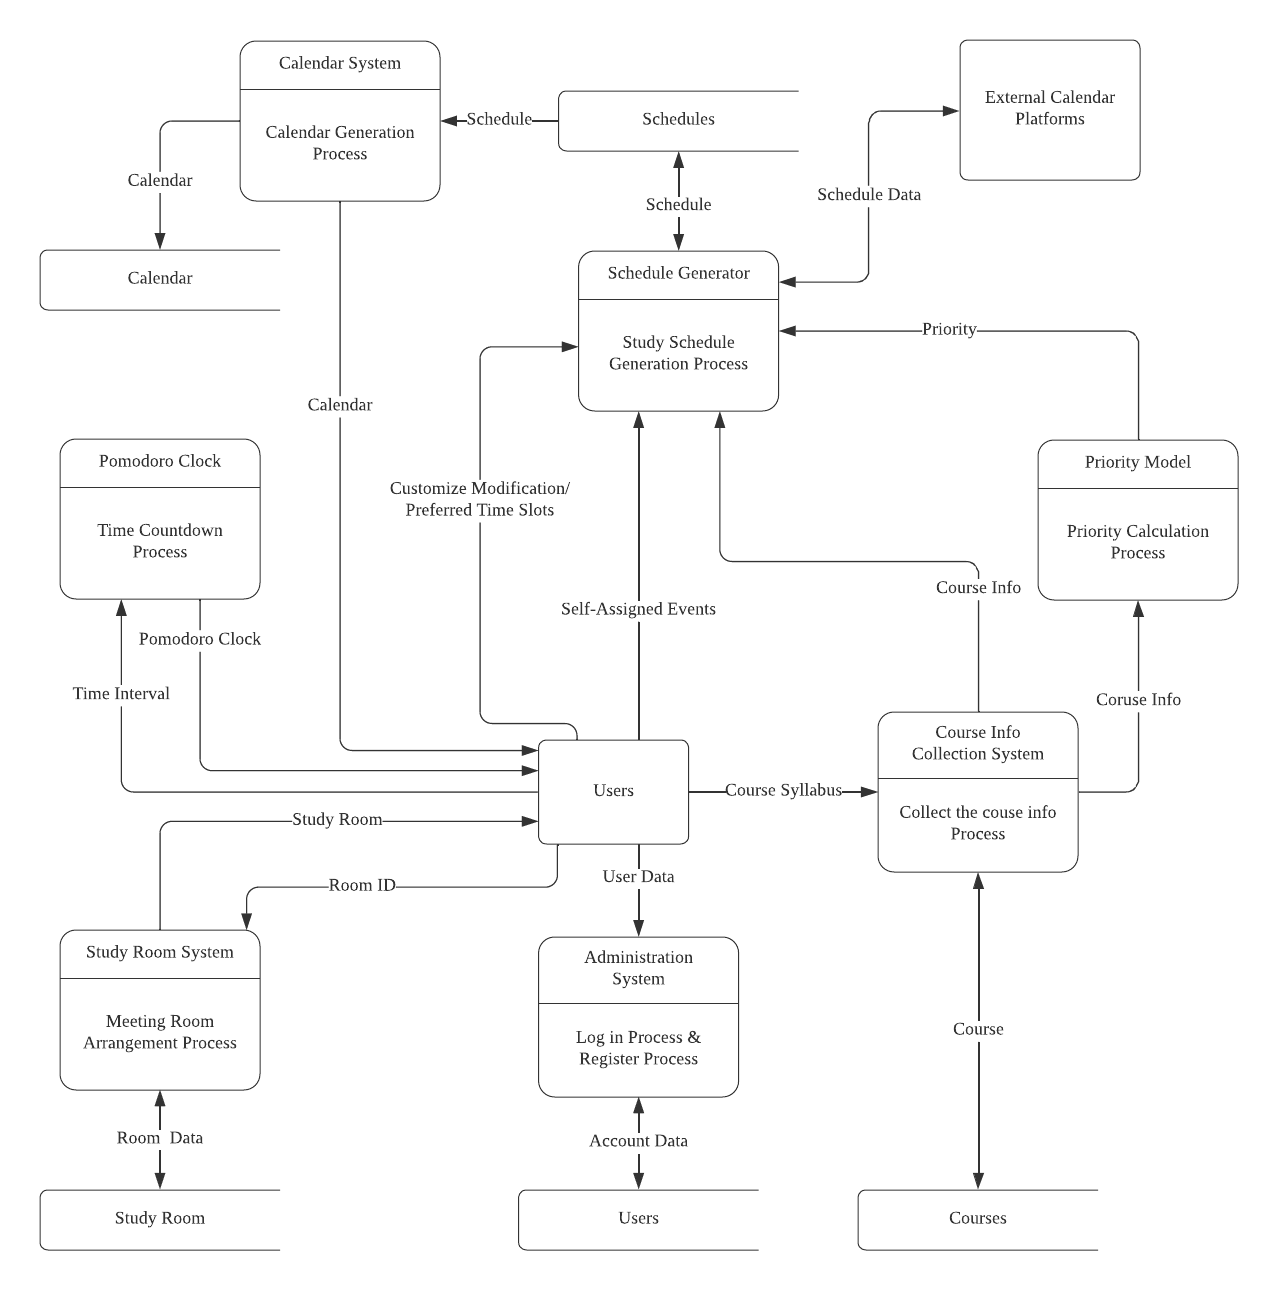
\includegraphics[width=0.8\textwidth]{DFD.png}
  \caption{Data Flow Diagram} 
  \label{fig:dfd} 
\end{figure}

\subsection{Data Dictionary}
\lips

\section{The Scope of the Product}

\subsection{Product Boundary}
The Smart Study Helper App aims to serve as a comprehensive solution for students to manage their study schedules and tasks effectively. Its boundary extends from user registration, task generation, and prioritization, to progress visualization and study planning. It will interact with external calendar services and will allow users to collaborate with peers through its social network component. However, the app’s boundary does not extend to managing non-academic tasks or any other aspects of a user’s daily life not related to their study.

\subsection{Product Use Case Table}
\begin{longtable}{ |p{3cm}|p{5cm}|p{5cm}|}
    \hline
    Use Case Name & Primary Actor & Description \\
    \hline
    User Registration & Student & Allows new users to create an account \\
    \hline
    Upload Syllabus & Student & Enables users to upload course syllabus in PDF format \\
    \hline
    Task Generation & Application & Automatically generates tasks based on uploaded syllabus \\
    \hline
    Task Prioritization & Application & Prioritizes tasks based on ML algorithms \\
    \hline
    Progress Visualization & Student & Users can view the status of their tasks \\
    \hline
    Facial Recognition & Application & Detect users' stress levels by recognizing users' face \\
    \hline
    Classmates Lookup & Student & Users can look up online classmates who register the same course \\
    \hline
    Connected Learning & Student & Users can connect with their friends or classmates to study together \\
    \hline
    User Login & Student & Allows users to log into their account using username and password \\
    \hline
    Friend List Management & Student & Supports friend list for sending/rejecting/accepting friend requests \\
    \hline
    Export to Other Calendars & Application, Student & Exports event and schedule data to third-party calendar apps \\
    \hline
    Estimate Task Duration & Application & Calculates the estimated time for each task from course outlines \\
    \hline
\end{longtable}

\subsection{Individual Product Use Cases (PUC’s)}
\begin{figure}[htbp]
    \centering
    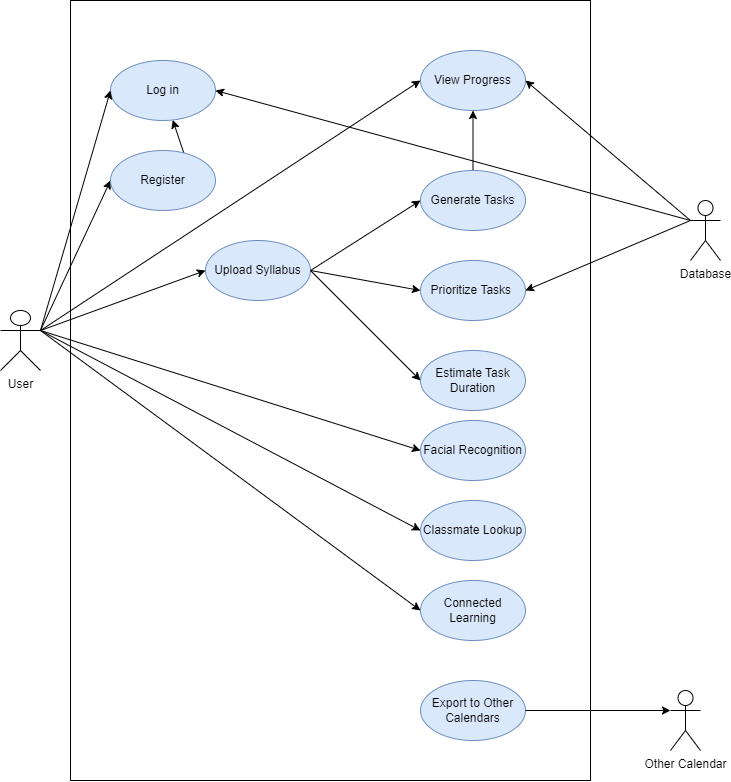
\includegraphics[width=0.7\linewidth]{Use Case Diagram.drawio.png} 
    \caption{Use Case Diagram}
    \label{fig:samplelabel}
\end{figure}

\subsubsection{User Registration}
\begin{itemize}
    \item \textbf{Goal:} Enable students to create a unique account.
    \item \textbf{Actors:} Student.
    \item \textbf{Preconditions:} Student has accessed the application or web.
    \item \textbf{Postconditions:} Student has an active account and can access the app's features.
    \item \textbf{Main Flow:} Student enters required information, sets a password, and completes registration.
\end{itemize}

\subsubsection{Upload Syllabus}
\begin{itemize}
    \item \textbf{Goal:} Allow students to upload their course syllabus.
    \item \textbf{Actors:} Student.
    \item \textbf{Preconditions:} Student is logged in.
    \item \textbf{Postconditions:} Syllabus is stored and ready for task generation.
    \item \textbf{Main Flow:} Student selects the course syllabus in PDF format and uploads it.
\end{itemize}

\subsubsection{Task Generation}
\begin{itemize}
    \item \textbf{Goal:} Create tasks from the uploaded syllabus.
    \item \textbf{Actors:} Application.
    \item \textbf{Preconditions:} Syllabus has been uploaded.
    \item \textbf{Postconditions:} Tasks are generated and displayed to the student.
    \item \textbf{Main Flow:} Application processes the syllabus and generates relevant tasks.
\end{itemize}

\subsubsection{Task Prioritization}
\begin{itemize}
    \item \textbf{Goal:} Rank tasks based on importance.
    \item \textbf{Actors:} Application.
    \item \textbf{Preconditions:} Tasks have been generated.
    \item \textbf{Postconditions:} Tasks are prioritized and presented in an organized manner.
    \item \textbf{Main Flow:} Application uses ML algorithms to analyze and prioritize tasks.
\end{itemize}

\subsubsection{Progress Visualization}
\begin{itemize}
    \item \textbf{Goal:} Offer students a view of their task progress.
    \item \textbf{Actors:} Student.
    \item \textbf{Preconditions:} Tasks have been generated and prioritized.
    \item \textbf{Postconditions:} Student can visually assess task status.
    \item \textbf{Main Flow:} Student accesses a dashboard or progress section to view status of tasks.
\end{itemize}

\subsubsection{Facial Recognition}
\begin{itemize}
    \item \textbf{Goal:} Identify student stress levels using facial cues.
    \item \textbf{Actors:} Application.
    \item \textbf{Preconditions:} Student grants camera access.
    \item \textbf{Postconditions:} App detects potential stress indicators.
    \item \textbf{Main Flow:} Application uses facial recognition technology to analyze student's face for stress signs.
\end{itemize}

\subsubsection{Classmates Lookup}
\begin{itemize}
    \item \textbf{Goal:} Allow students to find classmates in the same course.
    \item \textbf{Actors:} Student.
    \item \textbf{Preconditions:} Student is registered in a course.
    \item \textbf{Postconditions:} Student views a list of classmates in the same course.
    \item \textbf{Main Flow:} Student accesses course section and views registered classmates.
\end{itemize}

\subsubsection{Connected Learning}
\begin{itemize}
    \item \textbf{Goal:} Provide students with a platform to study collaboratively.
    \item \textbf{Actors:} Students.
    \item \textbf{Preconditions:} Students have active accounts.
    \item \textbf{Postconditions:} Students can connect and study together.
    \item \textbf{Main Flow:} A student sends a connection request to another student. Once accepted, they can access video chat with joint study tools and features.
\end{itemize}

\subsubsection{User Login}
\begin{itemize}
    \item \textbf{Goal:} Allow students to log into their account.
    \item \textbf{Actors:} Student.
    \item \textbf{Preconditions:} Student has an active account.
    \item \textbf{Postconditions:} Student is logged in and can access personalized data.
    \item \textbf{Main Flow:} Student provides username and password; if credentials match, access is granted.
\end{itemize}

\subsubsection{Friend List Management}
\begin{itemize}
    \item \textbf{Goal:} Manage friend connections within the application.
    \item \textbf{Actors:} Student.
    \item \textbf{Preconditions:} Student is logged in.
    \item \textbf{Postconditions:} Updated friend list status (friend request sent/received/accepted/rejected).
    \item \textbf{Main Flow:} Student navigates to the friend list section, sends/receives/accepts/rejects friend requests.
\end{itemize}

\subsubsection{Export to Other Calendars}
\begin{itemize}
    \item \textbf{Goal:} Export event and schedule data to third-party calendar apps.
    \item \textbf{Actors:} Application, Student.
    \item \textbf{Preconditions:} Student has events or schedules in the application.
    \item \textbf{Postconditions:} Events and schedules are exported and viewable in third-party apps.
    \item \textbf{Main Flow:} With authentication, student initiates export to a chosen calendar app; data is formatted and transferred.
\end{itemize}

\subsubsection{Estimate Task Duration}
\begin{itemize}
    \item \textbf{Goal:} Calculate the estimated time needed for each task from course outlines.
    \item \textbf{Actors:} Application.
    \item \textbf{Preconditions:} Tasks have been extracted from course outlines.
    \item \textbf{Postconditions:} Each task has an associated time estimate.
    \item \textbf{Main Flow:} Application processes tasks from course outlines and estimates time requirements for each.
\end{itemize}



\section{Functional Requirements}
\subsection{Functional Requirements}
\lips

\section{Look and Feel Requirements}

\subsection{Appearance Requirements}
The application's design should be user-friendly and intuitive. Key elements to consider include:
\paragraph{AR1:} Clear typography: Text should be legible at all standard screen resolutions and sizes. 
\paragraph{AR2:}Color scheme: The color palette should be eye-catching but not overwhelming. Calming and neutral tones should be used that helps to focus.
\paragraph{AR3:}Icons and graphics: Visual aids should be recognizable and easy to learn.
\paragraph{AR4:}Layout: The design should be responsive, ensuring usability across devices of varying screen sizes, from smartphones to tablets to desktop monitors.

\subsection{Style Requirements}
The style of the application should make the application easy and clear to use, providing a sense of community for students. Aspects to focus on include:
\paragraph{SR1:}Navigation: Menus and navigation tools should be logically organized and easy to access. 
\paragraph{SR2:}Consistency: Elements like buttons, text fields, and icons should maintain a consistent design throughout the application.
\paragraph{SR3:}Interactivity: Interactive elements like buttons or dropdowns should provide feedback, indicating appropriate responsiveness.
\paragraph{SR4:}Accessibility: The design should cater to all users, including those with disabilities and elder adults. Features like text-to-speech and adjustable font sizes should be considered.
\paragraph{SR5:}Animations: Any animations used should be subtle and not distractive so users can focus more on the main content. 



\section{Usability and Humanity Requirements}
\subsection{Ease of Use Requirements}
\lips
\subsection{Personalization and Internationalization Requirements}
\lips
\subsection{Learning Requirements}
\lips
\subsection{Understandability and Politeness Requirements}
\lips
\subsection{Accessibility Requirements}
\lips

\section{Performance Requirements}

\subsection{Speed and Latency Requirements}
\paragraph{SLR1:} Major actions, such as uploading syllabuses, generating tasks, and prioritizing tasks, should be completed in a timely manner.
\paragraph{Fit Criteria:} During testing under normal load conditions, major actions are executed within a 2-second threshold.

\subsection{Safety-Critical Requirements}
\paragraph{SCR1:} All data, especially sensitive academic information, must be securely encrypted to ensure protection against unauthorized access.
\paragraph{Fit Criteria:} Throughout security testing, no incidents of data breaches or unauthorized data accesses are observed.

\subsection{Precision or Accuracy Requirements}
\paragraph{PAR1:} ML-based features, particularly task prioritization, must achieve a high degree of accuracy.
\paragraph{Fit Criteria:} When tested against predefined scenarios, ML algorithms show an accuracy rate of 90\% in task categorization and prioritization.

\subsection{Robustness or Fault-Tolerance Requirements}
\paragraph{RFTR1:} The application must demonstrate resilience against unexpected inputs or actions and provide means of efficient data recovery.


\subsection{Capacity Requirements}
\paragraph{CR1:} The system should be robust enough to manage a large number of concurrent users.
\paragraph{Fit Criteria:} During load testing, the application manages the equivalent load of 10,000 users and data pertaining to 1 million courses without any performance issues or system crashes.
\paragraph{CR2:}The system should store vast quantities of course data without any compromise in performance.
\paragraph{Fit Criteria:} During load testing, the application manages the equivalent load of 1 million courses without any performance issues or system crashes.
\subsection{Scalability or Extensibility Requirements}
\paragraph{SER1:} The design and architecture of the application should support ease of modification and the addition of new features.


\subsection{Longevity Requirements}
N/A



\section{Operational and Environmental Requirements}
\subsection{Expected Physical Environment}
\lips
\subsection{Wider Environment Requirements}
\lips
\subsection{Requirements for Interfacing with Adjacent Systems}
\lips
\subsection{Productization Requirements}
\lips
\subsection{Release Requirements}
\lips

\section{Maintainability and Support Requirements}
\subsection{Maintenance Requirements}
\lips
\subsection{Supportability Requirements}
\lips
\subsection{Adaptability Requirements}
\lips

\section{Security Requirements}
\subsection{Access Requirements}
\lips
\subsection{Integrity Requirements}
\lips
\subsection{Privacy Requirements}
\lips
\subsection{Audit Requirements}
\lips
\subsection{Immunity Requirements}
\lips

\section{Cultural Requirements}
\subsection{Cultural Requirements}
\lips

\section{Compliance Requirements}
\subsection{Legal Requirements}
\lips
\subsection{Standards Compliance Requirements}
\lips

\section{Open Issues}
\lips

\section{Off-the-Shelf Solutions}
\subsection{Ready-Made Products}
\lips
\subsection{Reusable Components}
\lips
\subsection{Products That Can Be Copied}
\lips

\section{New Problems}
\subsection{Effects on the Current Environment}

\begin{itemize}
    \item The introduction of new time management tools may affect existing scheduling systems within educational organizations. Any changes to the way students manage the study schedule may affect the way teachers and administrators organize their workflow and thus their existing scheduling systems.

    \item The implementation of a new system may change the way students interact with existing tools and platforms. If the new tool enables seamless integration with existing popular scheduling platforms, users may stop using other scheduling tools. Some users may need to adapt to these changes, and this transition needs to be handled carefully to ensure a smooth user experience.

    \item The data security requirements of the new tool and the user access control may require changes to the current security infrastructure. Any potential impact on existing security protocols should be fully assessed, and measures taken to mitigate risks.

    \item The new system may change user workflows and procedures. If it automates and prioritizes tasks, this may impact the way they plan and manage assignment completion and course scheduling. Understanding and responding to these changes as early as possible is critical to ensure smooth operation.
\end{itemize}

\subsection{Effects on the Installed Systems}
This section specifies the interfaces between the new system and existing systems or components.
\begin{itemize}
    \item \textbf{Interface with Google Calendar}: The system should integrate with Google Calendar to synchronize and visualize task deadlines. The interface will involve certification, data exchange, and event management.
    
    \item \textbf{Interface with Outlook Calendar}: Similar to Google Calendar, the system shall integrate with Outlook Calendar to synchronize events. The interface will involve certification and event management.

    \item \textbf{Interface with Machine Learning Server}: The system relies on machine learning algorithms to prioritize tasks. This interface includes sending data to the machine learning server, processing suggestions, and integrating them into the user interface.

    \item \textbf{Interface to connect with users}: To facilitate collaborative learning, the system should enable users to connect with their peers. This interface includes user authentication, data exchange, and video chat integration.

    \item \textbf{Interface with videoconferencing hardware} Users will use webcams, microphones, and speakers for video chat during collaborative learning. This interface is required to access these hardware components and manage live video conferencing.
\end{itemize}
\subsection{Potential User Problems}
\begin{itemize}
    \item \textbf{User Confusion}:
    The addition of machine learning-driven task prioritization, facial recognition, and online collaborative learning session features may confuse or create resistance from some users who are unfamiliar with these concepts.
    
    \textbf{Prevention and mitigation measures:}
    \begin{itemize}
        \item Develop a user-friendly onboarding process and provide extensive training materials to ensure users can easily understand and use the new features.
        \item Provide customization options that allow users to customize the system to their preferences. This flexibility will help users take better control of their experience.
    \end{itemize}
    
    \item \textbf{Privacy Concerns}:
    Users may have privacy concerns, especially with attention-monitoring features such as facial recognition. They may be concerned that their facial data will be collected and used.
    
    \textbf{Prevention and Mitigation Measures:}
    \begin{itemize}
        \item Privacy concerns are addressed by implementing strong data protection measures. Users will be informed of what their data will be used for and how it will be processed and will be able to opt out of certain features.
    \end{itemize}
    
    \item \textbf{Technical Issues}:
    Technical issues or system incompatibilities may lead to adverse reactions, such as issues related to platform support or software bugs.
    
    \textbf{Prevention and Mitigation Measures:}
    \begin{itemize}
        \item Rigorous testing and quality assurance are conducted to detect and correct technical issues before they affect users. Updates and bug fixes will be performed regularly to ensure system stability.
    \end{itemize}
\end{itemize}

\subsection{Limitations in the Anticipated Implementation Environment That May
Inhibit the New Product}
\begin{itemize}
    \item The planned servers may not have enough processing power or storage capacity to handle the expected growth in users and data volume.
    
    \item Available network bandwidth may not be sufficient to support real-time videoconferencing for collaborative learning sessions, leading to potential performance issues.
    
    \item Implementing system integration with external calendaring platforms (e.g., Google Calendar, Outlook) takes into account that these platforms may have limitations or constraints that affect the quality of the integration.
    
    \item Hardware for facial recognition may not be readily available or may not meet the accuracy requirements for detecting the user's level of attention.
    
    \item The implementation environment may be subject to specific data privacy regulations that may affect the collection and storage of user data.
\end{itemize}

\subsection{Follow-Up Problems}
This section anticipates potential challenges, unintended consequences, and limitations that the project may encounter during development and implementation.

\begin{itemize}
    \item The implementation of new features or technologies in the system may inadvertently result in non-compliance with existing laws and regulations, such as user privacy protection aspect. The project team will conduct regular assessments. Any necessary changes will be made to address potential legal issues.
    \item 
\end{itemize}

\section{Tasks}
\subsection{Project Planning}
\href{https://github.com/wangq131/4G06CapstoneProjectT5/blob/main/docs/DevelopmentPlan/DevelopmentPlan.tex#L248C1-L265C6}{See Project Scheduling Section in Development Plan.}
\subsection{Planning of the Development Phases}
\href{https://github.com/wangq131/4G06CapstoneProjectT5/blob/main/docs/DevelopmentPlan/DevelopmentPlan.tex#L194C1-L245C16}{See Project Scheduling Section in Development Plan.}

\section{Migration to the New Product}
The project is a stand-alone application, not an upgrade or replacement of an existing product. There is no need to involve a product migration. The Migration to the New Product section is not needed.

\section{Costs}
The following are some of the major cost items that may need to be considered:

\begin{itemize} 
  \item \textbf{Cloud services}: using a cloud infrastructure (e.g. \textit{Amazon AWS}, \textit{Microsoft Azure}, or \textit{Google Cloud}) requires consideration of the cost of using cloud services.
  \item \textbf{Server hosting}: using an independent server, server hosting, and maintenance costs need to be considered.
  \item \textbf{Database}: database storage and access costs.
  \item \textbf{Data Backup}: regular data backup and storage costs.
  \item \textbf{Working Time}: takes NUMBER\_Of\_MEMBERS group members WORK\_HOURS a week.
\end{itemize}

\section{User Documentation and Training}
\subsection{User Documentation Requirements}
\lips
\subsection{Training Requirements}
\lips

\section{Waiting Room}
\lips

\section{Ideas for Solution}
\lips

\newpage{}
\section*{Appendix --- Reflection}

The information in this section will be used to evaluate the team members on the
graduate attribute of Lifelong Learning.  Please answer the following questions:

\begin{enumerate}
  \item What knowledge and skills will the team collectively need to acquire to
  successfully complete this capstone project?  Examples of possible knowledge
  to acquire include domain specific knowledge from the domain of your
  application, or software engineering knowledge, mechatronics knowledge or
  computer science knowledge.  Skills may be related to technology, or writing,
  or presentation, or team management, etc.  You should look to identify at
  least one item for each team member.
  \item For each of the knowledge areas and skills identified in the previous
  question, what are at least two approaches to acquiring the knowledge or
  mastering the skill?  Of the identified approaches, which will each team
  member pursue, and why did they make this choice?
\end{enumerate}

\end{document}